% Metódy inžinierskej práce

\documentclass[10pt,twoside,slovak,a4paper]{coursepaper}

\usepackage[slovak]{babel}
%\usepackage[T1]{fontenc}
\usepackage[IL2]{fontenc} % lepšia sadzba písmena Ľ než v T1
\usepackage[utf8]{inputenc}
\usepackage{graphicx}
\usepackage{url} % príkaz \url na formátovanie URL
\usepackage{hyperref} % odkazy v texte budú aktívne (pri niektorých triedach dokumentov spôsobuje posun textu)

\usepackage{todonotes}
\usepackage{pdfpages}

\usepackage{cite}
%\usepackage{times}

\pagestyle{headings}

\title{Is Netflix recommendation system a problem ?\thanks{Semestrálny projekt v predmete Metódy inžinierskej práce, ak. rok 2024/2025, vedenie: Mgr. Yevheniia Kataieva, PhD.}}

\author{Adam Glogovský\\[2pt]
	{\small Slovenská technická univerzita v Bratislave}\\
	{\small Fakulta informatiky a informačných technológií}\\
	{\small \texttt{xglogovsky@stuba.sk}}
	}

\date{\small 30. september 2024} % upravte



\begin{document}

\maketitle

\begin{abstract}
	Touto prácou by som chcel poukázať na to, ako Netflix ako firma spracúva užívateľské informácie. Kde tieto informácie posiela. Ako ich spracúva a ako podľa nich dokáže nám užívateľom spríjemniť fungovanie na platforme. Ak nám to zvyšuje zážitok z používania tejto platformy, čo to teda tú platformu stojí a či je to vo výsledku pre danú platformu efektívne a finančne prospešné. Taktiež sa pokúsim čo naviac priblížiť samotné spracovanie týchto údajov a poukážem na to, či je správne daným spôsobom spracúvať tieto informácie.\cite{amatriain2015recommender} Dôležítý taktiež pre platformu je, algoritmus akým spracúvajú dané informácie a infraštruktúra v ktorej to celé funguje. Samozrejme zistiť, či kvôli tomuto alogritmu a spôsobu spracovania informácií, neubližujú menej populárnemu obsahu, ktorý je teda ešte o to menej ukazovaný užívateľom. A tiež poukážem na to, či je tento menej populárny obsah iba nefavoritizovaný alebo je kompletne zahaľovaný určitým užívateľom.
	\todo[color=blue!15]{Adam: 142 slov}
\end{abstract}



\section{Úvod}

Motivujte čitateľa a vysvetlite, o čom píšete. Úvod sa väčšinou nedelí na časti.

Uveďte explasdôlkfasicitne štruklksdjfklsfôsdfôaltúru článku. Tu je nejaký príklad.
Základný problém, ktorý bol naznačený v úvode, je podrobnejšie vysvetlený v časti~\ref{nejaka}.
Dôležité súvislosti sú uvedené v častiach~\ref{dolezita} a~\ref{dolezitejsia}.
Záverečné poznámky prináša časť~\ref{zaver}.

\section{Toto je nová sekcia} \label{pouziva sa pre referencie}
\input{novy.txt}
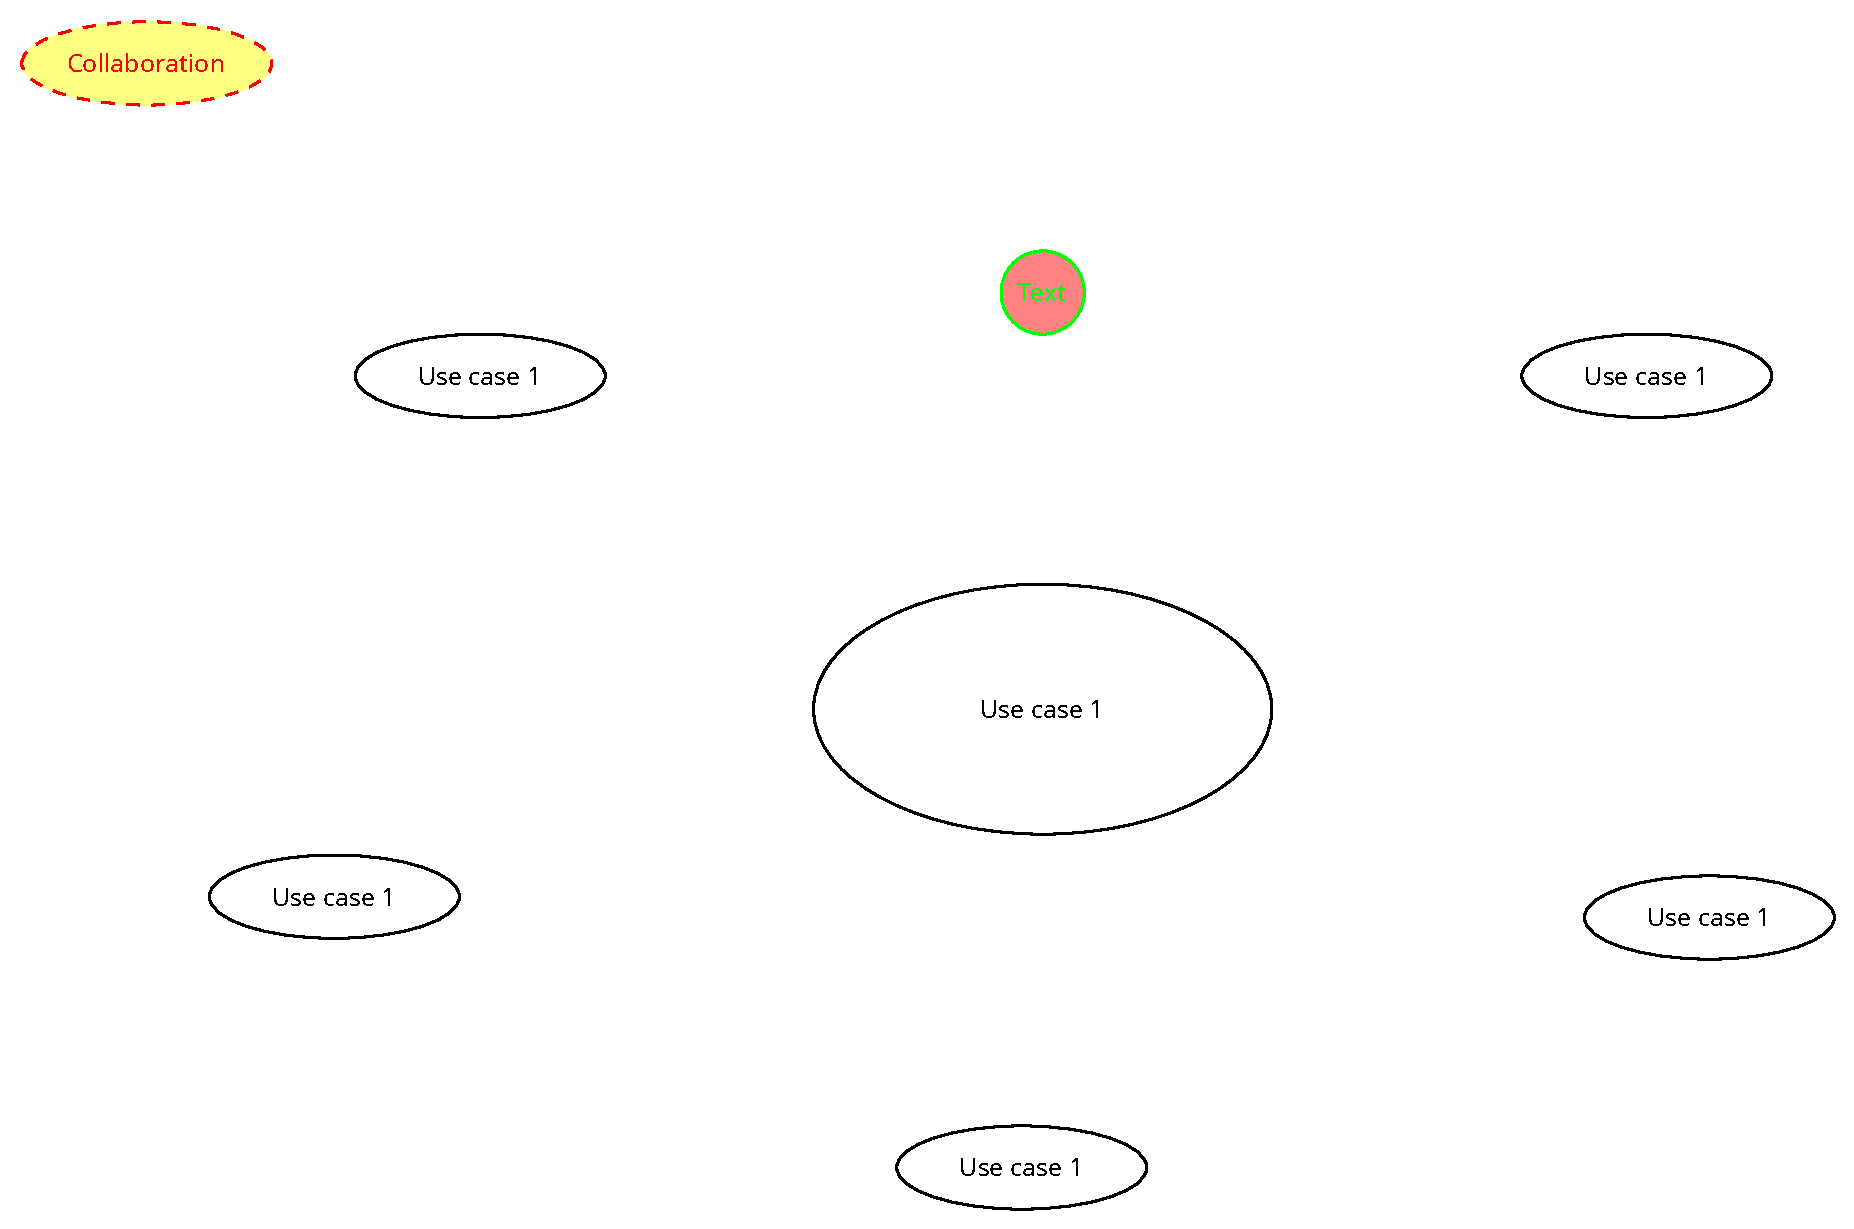
\includepdf{diagram.pdf}

\section{Nejaká časť} \label{nejaka}

Z obr.~\ref{f:rozhod} je všetko jasné.

\begin{figure*}[tbh]
	\centering
	%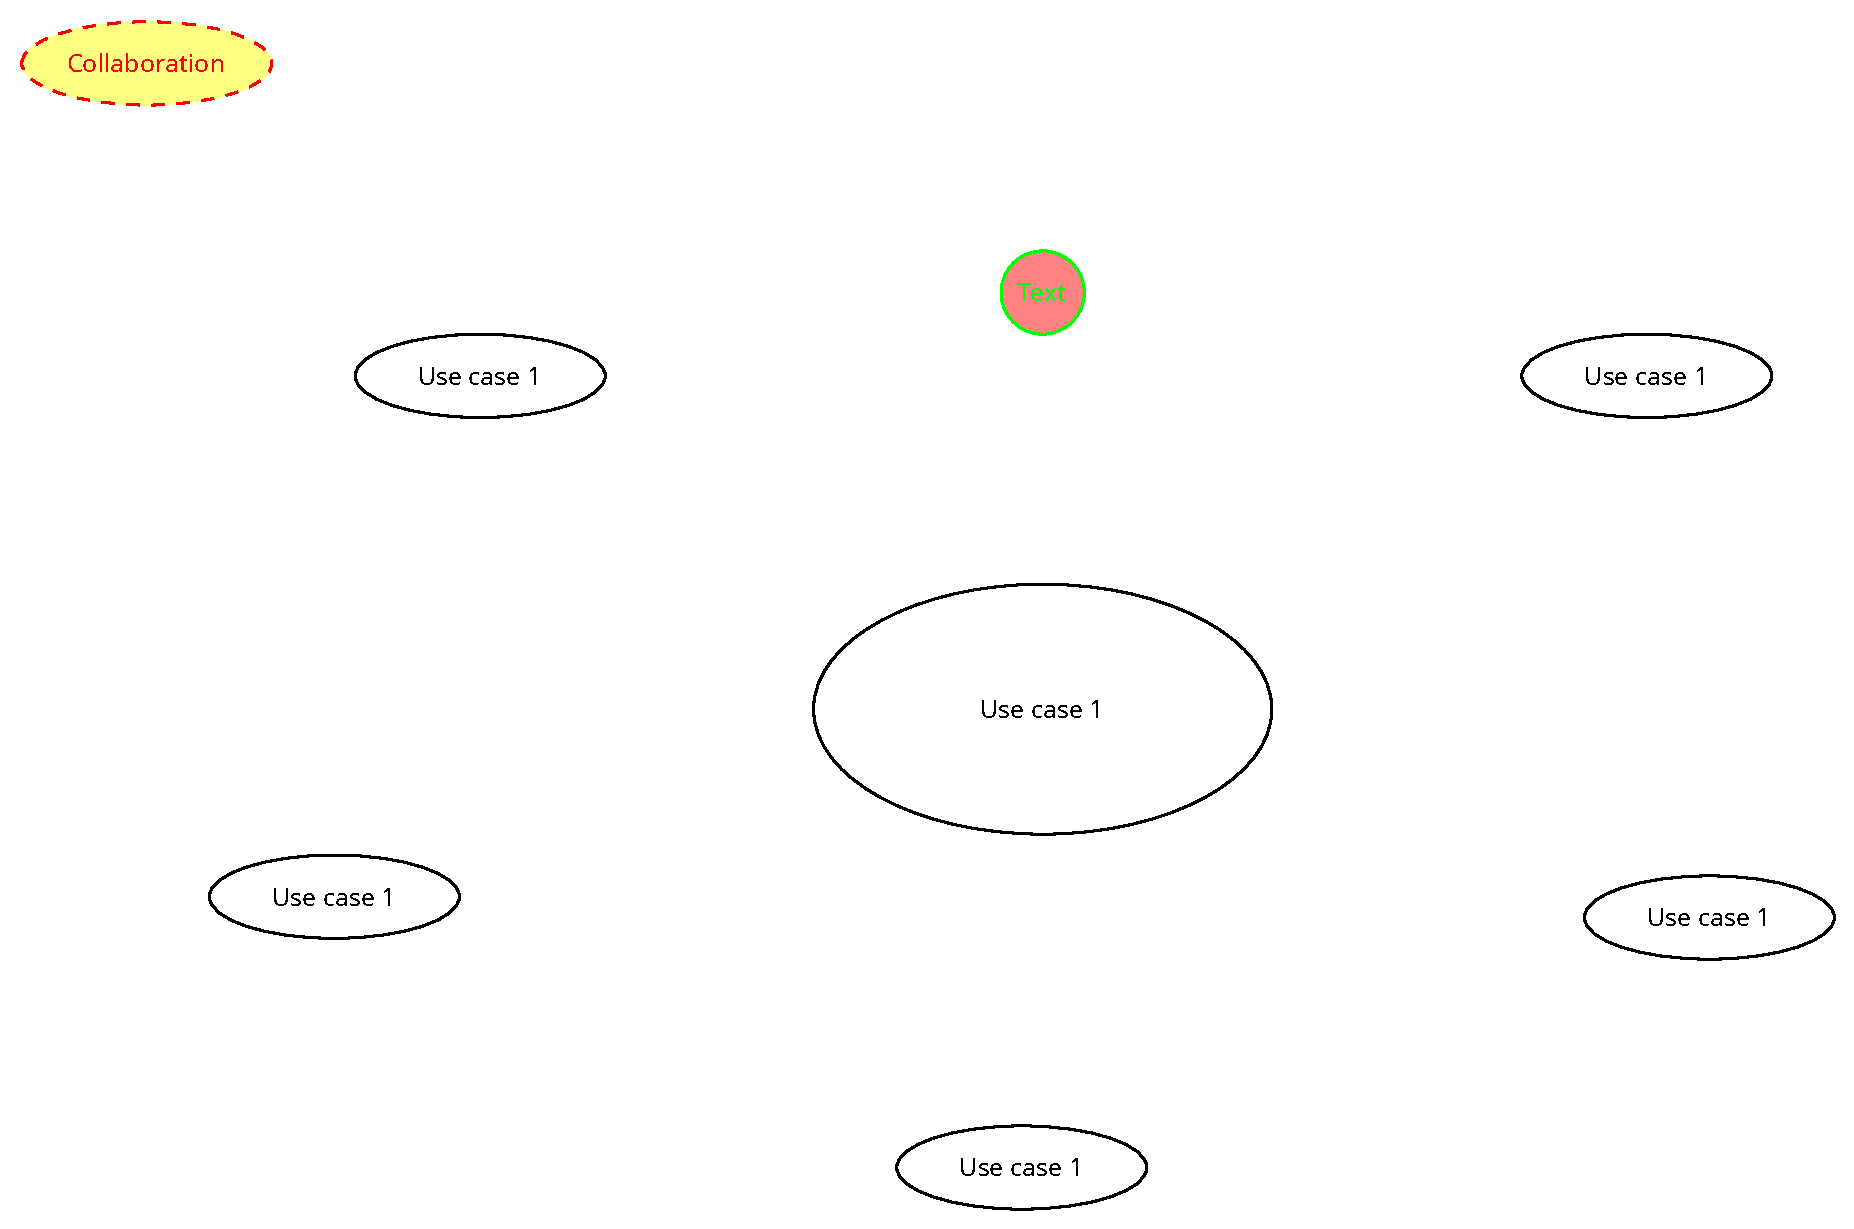
\includegraphics[scale=1.0]{diagram.pdf}
	Aj text môže byť prezentovaný ako obrázok. Stane sa z neho označný plávajúci objekt. Po vytvorení diagramu zrušte znak \texttt{\%} pred príkazom \verb|\includegraphics| označte tento riadok ako komentár (tiež pomocou znaku \texttt{\%}).
	\caption{Rozhodujúci argument.}
	\label{f:rozhod}
\end{figure*}



\section{Iná časť} \label{ina}

Základným problémom je teda\ldots{} Najprv sa pozrieme na nejaké vysvetlenie (časť~\ref{ina:nejake}), a potom na ešte nejaké (časť~\ref{ina:nejake}).\footnote{Niekedy môžete potrebovať aj poznámku pod čiarou.}

Môže sa zdať, že problém vlastne nejestvuje\cite{Coplien:MPD}, ale bolo dokázané, že to tak nie je~\cite{Czarnecki:Staged, Czarnecki:Progress}. Napriek tomu, aj dnes na webe narazíme na všelijaké pochybné názory\cite{PLP-Framework}. Dôležité veci možno \emph{zdôrazniť kurzívou}. dalsia vec ktoru citujem \cite{Steck_Baltrunas_Elahi_Liang_Raimond_Basilico_2021}


\subsection{Nejaké vysvetlenie} \label{ina:nejake}

Niekedy treba uviesť zoznam:

\begin{itemize}
	\item jedna vec
	\item druhá vec
	      \begin{itemize}
		      \item x
		      \item y
	      \end{itemize}
\end{itemize}

Ten istý zoznam, len číslovaný neisty zoznam:

\begin{enumerate}
	\item jedna vec
	\item druhá vec
	      \begin{enumerate}
		      \item x
		      \item y
	      \end{enumerate}
\end{enumerate}


\subsection{Ešte nejaké vysvetlenie} \label{ina:este}

\paragraph{Veľmi dôležitá poznámka.}
Niekedy je potrebné nadpisom označiť odsek. Text pokračuje hneď za nadpisom.



\section{Dôležitá časť} \label{dolezita}




\section{Ešte dôležitejšia časť} \label{dolezitejsia}




\section{Záver} \label{zaver} % prípadne iný variant názvu



%\acknowledgement{Ak niekomu chcete poďakovať\ldots}


% týmto sa generuje zoznam literatúry z obsahu súboru literatura.bib podľa toho, na čo sa v článku odkazujete
\bibliography{literatura}
\bibliographystyle{abbrv} % prípadne alpha, abbrv alebo hociktorý iný
\end{document}
